\chapter{Continuidad}

\section{Funciones Continuas}

\begin{definition}
	Sean $(X, d_X)$ e $(Y, d_Y)$ espacios métricos. Una función $f : X \to Y$ se dice \emph{continua en} $x$ si
	\begin{center}
		\begin{minipage}{0.9\linewidth}
			para todo $\varepsilon > 0$, existe un $\delta > 0$ tal que $d_X (x', x) < \delta$ implica $d_Y (f(x'), f(x)) < \varepsilon$, para todo $x' \in X$.
		\end{minipage}
	\end{center}
	Decimos que $f$ es \emph{continua} si es continua en todo punto de su dominio.
\end{definition}

\begin{remark}
	O más compacto:
	\begin{equation*}
		\forall \varepsilon > 0, \exists \delta > 0 \mid d_X (x', x) < \delta \Rightarrow d_Y (f(x'), f(x)), \forall x' \in X.
	\end{equation*}
\end{remark}

Es muy útil pensar la continuidad de forma intuitiva utilizando la noción de entornos. Si $f$ es continua en $x$, entonces para todo entorno $V$ de $f(x)$, $f^{-1}(V)$ es un entorno de $x$.

\begin{center}
	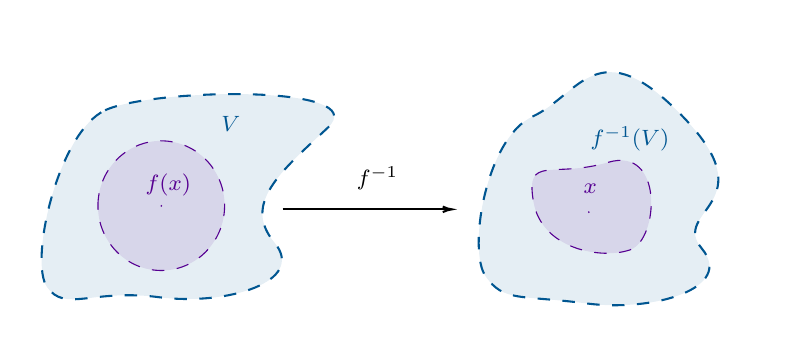
\begin{tikzpicture}[x=0.75pt,y=0.75pt,yscale=-1,xscale=1]
	%uncomment if require: \path (0,300); %set diagram left start at 0, and has height of 300

	%Shape: Polygon Curved [id:ds9863252903529107] 
	\draw  [color={rgb, 255:red, 0; green, 86; blue, 145 }  ,draw opacity=1 ][fill={rgb, 255:red, 0; green, 86; blue, 145 }  ,fill opacity=0.1 ][dash pattern={on 4.5pt off 4.5pt}][line width=0.75]  (57.97,33.79) .. controls (80.65,23.22) and (187.88,21.11) .. (165.2,42.24) .. controls (142.52,63.36) and (123.85,78.74) .. (139.52,97.54) .. controls (155.2,116.35) and (116.63,128.1) .. (84,123.88) .. controls (51.37,119.65) and (38.86,131.38) .. (30,119) .. controls (21.14,106.62) and (35.29,44.35) .. (57.97,33.79) -- cycle ;
	%Shape: Ellipse [id:dp7045194170512884] 
	\draw  [color={rgb, 255:red, 86; green, 0; blue, 145 }  ,draw opacity=1 ][fill={rgb, 255:red, 86; green, 0; blue, 145 }  ,fill opacity=0.1 ][dash pattern={on 4.5pt off 4.5pt}] (54.5,79.77) .. controls (54.5,62.52) and (68.16,48.54) .. (85.01,48.54) .. controls (101.86,48.54) and (115.52,62.52) .. (115.52,79.77) .. controls (115.52,97.02) and (101.86,111) .. (85.01,111) .. controls (68.16,111) and (54.5,97.02) .. (54.5,79.77) -- cycle ;
	%Shape: Ellipse [id:dp17380935073260606] 
	\draw  [color={rgb, 255:red, 86; green, 0; blue, 145 }  ,draw opacity=1 ][dash pattern={on 4.5pt off 4.5pt}] (84.91,79.87) .. controls (84.91,79.82) and (84.96,79.77) .. (85.01,79.77) .. controls (85.07,79.77) and (85.11,79.82) .. (85.11,79.87) .. controls (85.11,79.93) and (85.07,79.98) .. (85.01,79.98) .. controls (84.96,79.98) and (84.91,79.93) .. (84.91,79.87) -- cycle ;

	%Straight Lines [id:da5395275905863334] 
	\draw [line width=0.75]    (143.52,81.54) -- (223,81.54) ;
	\draw [shift={(225,81.54)}, rotate = 180] [color={rgb, 255:red, 0; green, 0; blue, 0 }  ][line width=0.75]    (4.37,-1.32) .. controls (2.78,-0.56) and (1.32,-0.12) .. (0,0) .. controls (1.32,0.12) and (2.78,0.56) .. (4.37,1.32)   ;
	%Shape: Polygon Curved [id:ds45640730182556577] 
	\draw  [color={rgb, 255:red, 0; green, 86; blue, 145 }  ,draw opacity=1 ][fill={rgb, 255:red, 0; green, 86; blue, 145 }  ,fill opacity=0.1 ][dash pattern={on 4.5pt off 4.5pt}][line width=0.75]  (263.97,36.79) .. controls (286.65,26.22) and (295.46,-5.49) .. (336.33,36.88) .. controls (377.2,79.24) and (329.85,81.74) .. (345.52,100.54) .. controls (361.2,119.35) and (322.63,131.1) .. (290,126.88) .. controls (257.37,122.65) and (250.2,126.26) .. (241.33,113.88) .. controls (232.47,101.49) and (241.29,47.35) .. (263.97,36.79) -- cycle ;
	%Shape: Ellipse [id:dp21595437817711993] 
	\draw  [color={rgb, 255:red, 86; green, 0; blue, 145 }  ,draw opacity=1 ][dash pattern={on 4.5pt off 4.5pt}] (290.91,82.87) .. controls (290.91,82.82) and (290.96,82.77) .. (291.01,82.77) .. controls (291.07,82.77) and (291.11,82.82) .. (291.11,82.87) .. controls (291.11,82.93) and (291.07,82.98) .. (291.01,82.98) .. controls (290.96,82.98) and (290.91,82.93) .. (290.91,82.87) -- cycle ;
	%Shape: Polygon Curved [id:ds49186281368908624] 
	\draw  [color={rgb, 255:red, 86; green, 0; blue, 145 }  ,draw opacity=1 ][fill={rgb, 255:red, 86; green, 0; blue, 145 }  ,fill opacity=0.1 ][dash pattern={on 4.5pt off 4.5pt}] (300.33,58.88) .. controls (327.33,50.88) and (324.67,96.13) .. (311,101) .. controls (297.33,105.88) and (268.33,100.88) .. (264.33,77.88) .. controls (260.33,54.88) and (273.33,66.88) .. (300.33,58.88) -- cycle ;

	% Text Node
	\draw (112.65,35.65) node [anchor=north west][inner sep=0.75pt]  [font=\footnotesize,color={rgb, 255:red, 0; green, 86; blue, 145 }  ,opacity=1 ]  {$V$};
	% Text Node
	\draw (76.25,63) node [anchor=north west][inner sep=0.75pt]  [font=\footnotesize,color={rgb, 255:red, 0; green, 145; blue, 105 }  ,opacity=1 ]  {$\textcolor[rgb]{0.34,0,0.57}{f( x)}$};
	% Text Node
	\draw (178,60) node [anchor=north west][inner sep=0.75pt]  [font=\footnotesize]  {$f^{-1}$};
	% Text Node
	\draw (290.65,40.65) node [anchor=north west][inner sep=0.75pt]  [font=\footnotesize,color={rgb, 255:red, 0; green, 86; blue, 145 }  ,opacity=1 ]  {$f^{-1}( V)$};
	% Text Node
	\draw (287.25,68) node [anchor=north west][inner sep=0.75pt]  [font=\footnotesize,color={rgb, 255:red, 86; green, 0; blue, 145 }  ,opacity=1 ]  {$x$};


\end{tikzpicture}

\end{center}

Veamos equivalencias de continuidad.

\begin{proposition}
	Sea $f : X \to Y$ y sea $x \in X$. Entonces, son equivalentes:
	\begin{enumerate}
		\item $f$ es continua en $x$.
		\item Si $x_n \longrightarrow x$, entonces $f(x_n) \longrightarrow f(x)$.
		\item Si $V \subseteq Y$ es un entorno de $f(x)$, entonces $f^{-1} (V)$ es un entorno de $x$.
	\end{enumerate}
\end{proposition}

Cuando decimos que una función $f$ es continua, nos referimos a que $f$ es continua en todo punto de su dominio.

\begin{proposition}
	Sea $f : X \to Y$. Entonces, son equivalentes:
	\begin{enumerate}
		\item $f$ es continua.
		\item Si $x_n \longrightarrow x$, entonces $f(x_n) \longrightarrow f(x)$ para todo $x \in X$ y sucesión $(x_n)_{n \in \mathbb{N}}$.
		\item $f^{-1} (A) \subseteq X$ es abierto para todo $A \subseteq Y$ abierto.
		\item $f^{-1} (B) \subseteq X$ es cerrado para todo $B \subseteq Y$ cerrado.
		\item $f( \overline{C} ) \subseteq \overline{f(C)}$ para todo $B \subseteq X$.
	\end{enumerate}
\end{proposition}

\begin{proof}
	\color{red} COMPLETAR
\end{proof}

\begin{proposition}
	La composición de funciones continuas es continua.
\end{proposition}

\section{Continuidad Uniforme}

\begin{definition}
	Decimos que $f : X \to Y$ es \emph{uniformemente continua} si
	\begin{equation*}
		\begin{split}
			\forall \varepsilon > 0, \exists \delta > 0 \text{ tal que } & d_X(x,x') < \delta \\ &\Rightarrow d_Y(f(x), f(x')) < \varepsilon, \forall x, x' \in X.
		\end{split}
	\end{equation*}
\end{definition}

\begin{remark}
	Las funciones uniformemente continuas mandan sucesiones de Cauchy a sucesiones de Cauchy.
\end{remark}

\begin{proposition}
	Sean $f, g : X \to Y$ continuas tales que $f |_A = g|_A$ con $A \subseteq X$ denso. Entonces, $g = g'$ en $X$.
\end{proposition}

\begin{proof}
	Sea $\Phi (x) = d(f(x), g(x))$. Por composición de funciones continuas, $\Phi$ es continua. Como $A \subseteq \Phi^{-1}(0)$ y $\left\{ 0 \right\}$ es cerrado, entonces $d(f(x), g(x)) = 0$ para todo $x \in \overline{D}$. Es decir, $f(x) = g(x)$ para todo $x \in X$.
\end{proof}


\section{Homeomorfismos}

Los homeomorfismo de cierta forma ``preservan'' la topología de un espacio.

\begin{definition}
	Decimos que $f : X \to Y$ es un \emph{homeomorfismo} si
	\begin{itemize}
		\item $f$ es continua.
		\item $f$ es biyectiva.
		\item $f^{-1}$ es continua.
	\end{itemize}
	Si existe un homeomorfismo de $X$ a $Y$, entonces decimos que son espacios \emph{homeomorfos}.
\end{definition}

También, definimos otros términos.

\begin{definition}
	Decimos que $f : X \to Y$ es
	\begin{itemize}
		\item \emph{abierta} si $f(A) \subseteq Y$ es abierto para todo $A \subseteq X$ abierto.
		\item \emph{cerrada} si $f(B) \subseteq Y$ es cerrado para todo $B \subseteq X$ cerrado.
	\end{itemize}
\end{definition}

\begin{remark}
	Son equivalentes
	\begin{itemize}
		\item homeomorfismo.
		\item continua y abierta.
		\item continua y cerrada.
	\end{itemize}
\end{remark}

\begin{example}
	Los espacios $\mathbb{R}$ y $(0, 1)$ son homeomorfos con la métrica usual.
\end{example}

En general, la idea de los homeomorfismos es que, de cierta forma, nos dicen que dos espacios métricos tienen las mismas propiedades. Por lo tanto, las propiedades \textit{topológicas} se mantienen con homeomorfismos. Es decir, los conceptos de abiertos, cerrados, puntos de acumulación, densos, continuidad sólo dependen de los abiertos y no la distancia del espacio métrico. (Esto lo habíamos visto antes y es la topología.)




